
\newpage
\section{Лекция 3}
\subsection{Полиномиальная интерполяция}
\textbf{Дано:} \\$f(x)$ --- неизвестный многочлен степени $\leq$ $n$\\
$f(x) = a_{0}+a_1x+...+a_nx^n$ \\
Известны значения $f(x)$ в точках $x_0, ..., x_n$ (всего $n+1$ значений)\\ 
$
\left\{  
\begin{array}{ccl}  
y_0=f(x_0)\\
\cdots\\
y_n=f(x_n)\\  
\end{array}   
\right.  
$
\\
\\ \textbf{Найти:} $f(x)$
\\ \textbf{Ответ:} \textbf{многочлен Лагранжа} \\
\begin{equation*}
\begin{cases}
a_0+a_1x_0+...+a_nx_0^n = y_0\\
\cdots\\
a_0+a_1x_n+...+a_nx_n^n = y_n
\end{cases}
\end{equation*}

\[\begin{pmatrix}
1 & x_0 & ... & x_0^n \\
\hdotsfor[1]{4} \\
1 & x_n & ... & x_n^n
\end{pmatrix} \cdot \begin{pmatrix}
a_0 \\
\vdots\\
a_n
\end{pmatrix} = \begin{pmatrix}
y_0 \\
\vdots\\
y_n
\end{pmatrix}\]
\textbf{Матрица Вандермонда}: $V(x_0,...,x_n)=V$ 
\begin{center}$V \bar a = \bar y$, $\bar a=V^{-1} \bar y$\end{center}
\textbf{Определитель Вандермонда}: $v(x_0,...,x_n) = det V(x_0,...,x_n) = (x_1-x_0)(x_2-x_0)...(x_n--x_0)(x_2-x_1)...(x_n-x_1)...(x_n-x_{n-1}) = \prod\limits_{0 \leq i < j \leq n} (x_j-x_i)$ 
\[ V = \begin{vmatrix}
1 & x_0 & ... & x_0^n \\
\hdotsfor[1]{4} \\
1 & x_n & ... & x_n^n
\end{vmatrix} = \begin{vmatrix}
1 & x_0 & ... & x_0^n \\
0 & x_1-x_0 & ... & x_1^n-x_0^n \\
\hdotsfor[2]{4} 
\end{vmatrix}\]
\begin{center}
    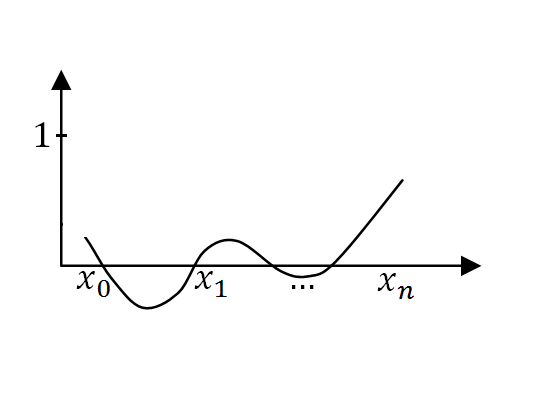
\includegraphics[scale=0.5]{l3_1.png}
\end{center}
\textbf{Многочлен Лагранжа}: \begin{center}$f(x)=L(x) = \sum\limits_{i=0}^{n} y_i \cdot \cfrac{\prod\limits_i (x-x_j)}{\prod\limits_j (x_i-x_j)} = \cfrac{\sum\limits_{i=0}^n y_i v(x_0,..., \underset{i}{x},..., x_n)}{v(x_0,..., x_n)}.$\end{center}
\noindent \textbf{Пример 1.}\\
Дано:\\
$x_0 = -1$, $x_1 = 0$, $x_2 = 1$\\
$y_0 = -2$, $y_1 = -1$, $y_2 = 2$\\
Провести параболу через три точки. Найти $f(x) = L(x) = a_0+a_1x+a_2x^2$.\\
\begin{center} $f(x) = \cfrac{-2(0-x)(1-x)+(-1)(x+1)(1+1)(1-x)+2(0+1)(x+1)(x-0)}{(0+1)(1+1)(1-0)} =$\\~\\$= x^2+2x-1$ \end{center}
\begin{center}
    $f(x) = (x-1)g(x) \Leftrightarrow f(1) = 0$\\
    $f(x) = (x-1)^2g(x) \Leftrightarrow$ 
    $  
    \left\{  
    \begin{array}{lcl}  
    f(1) = 0 \\  
    f'(1) = 0 \\  
    \end{array}   
    \right.  
    $
    \\
    $f'(x) = 2(x-1)g(x)+(x-1)^2g'(x)$
\end{center}

\begin{lemma}
\begin{center}
    $f(x) = (x-x_1)^kg(x) \Leftrightarrow$ 
    $  
    \left\{  
    \begin{array}{lcl}  
    f(x_1) = 0 \\  
    f'(x_1) = 0 \\
    \cdots\\
    f^{(k-1)}(x_1) = 0\\
    \end{array}   
    \right.  
    $
\end{center}
\end{lemma}

\subsection{Интерполяция с кратными узлами}
\textbf{Задача (кратко):}
Восстановить многочлен $f(x)$ по значениям в $m$ точках кратностей $k_1,..., k_m$.\\
\textbf{Формулировка:}
Найти многочлен $f(x)$ степени $\leq$ $n-1$ такой, что для некоторых различных узлов $x_1,...,x_m$ и некоторых натуральных $k_1,...,k_m$ (кратностей) верно\\
$  
\left\{  
\begin{array}{lcl}  
f(x_1) = y_1, f'(x_1) = y_1^{(1)},...,f^{(k_1-1)}(x_1) = y_1^{(k_1-1)} \\  
...\\
f(x_m) = y_m, f'(x_m) = y_m^{(1)},...,f^{(k_m-1)}(x_m) = y_m^{(k_m-1)} \\
\end{array}   
\right.  
$
\\ \\
Количество условий равно количеству неизвестных $k_1+...+k_m = n$.\\
\textbf{Ответ:} Многочлен Эрмита (или Лагранжа-Сильвестра).\\
\\
\begin{statement}
Такой многочлен существует и он единственный при $k_1+...+k_m = n$.
\end{statement}
Примечание: Если $k_1 = ... = k_m = 1$, то $m = n$ и $f(x)$ - многочлен Лагранжа (то есть предыдущий случай).\\
\begin{proof}
Пусть существует два таких многочлена $f(x)$ и $g(x)$, то для $p(x) = f(x)-h(x)$
\begin{center}
    $p^{(t)}(x_i) = 0, i=1,...,m, t\leq k_i$\\
    $p(x) = C(x-x_1)^{k_1}...(x-x_k)^{k_k} = C$ (многочлен степени $n+1$)\\
    $\Rightarrow C = 0, p(x) = 0$
\end{center}
Значит, если $f(x)$ существует, то он единственный.\\
Если $f(x) = a_0+a_1x+...+a_{n-1}x^{n-1}$, то \\
\[A \begin{pmatrix}[l]
~a_0 \\
~a_1 \\
~\vdots\\
~a_{n-1}
\end{pmatrix} = \begin{pmatrix}[l]
~y_0 \\
~y_2^{(1)}\\
~\vdots\\
~y_m^{(k_m-1)}
\end{pmatrix}\]\\
То есть, доказали, что система для любого $\bar y$ имеет не больше одного решения $\bar a$.\begin{center}
    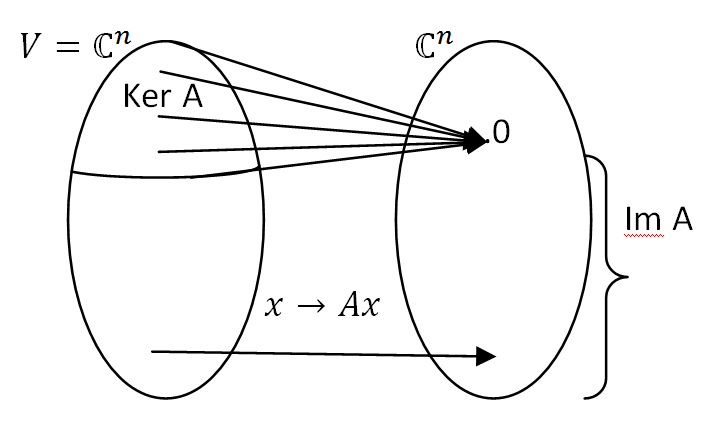
\includegraphics[scale=0.4]{l3_2.png}\end{center}
$Im A = \{ A \bar x | x\in \mathbb{C}^n \} $, 
$Ker A = \{\bar a | A \bar a = \bar 0 \} = \{\bar 0 \} $, так как у системы $A \bar a = \bar 0$ не больше одного решения.\\
Так как $A$ $n \times n$, то 
$dim(Im A) = rk A$, $dim(Ker A) = n-rk A$.\\ 
$Ker~ 0 \Leftrightarrow dim(Ker A) = 0$, то есть $rk A = n$ ($A$ невырожденная). \\
Матрица $A$ невырожденная $\Leftrightarrow$ $rk A = n \Leftrightarrow Im A = \mathbb{C}^n \Leftrightarrow Ker A = 0$, значит, $\bar a = A^{-1}\bar y$, всегда существует решение. 
\end{proof}
\subsection{Сплайны}
\noindent \textbf{1. Квадратичный.}\\
Надо установить функцию $f(x)$.\\
Аппроксимация: соседние точки надо соединить прямыми (не плавно). Но мы хотим гладко, значит на каждом отрезке надо задать свою функцию.\begin{center} 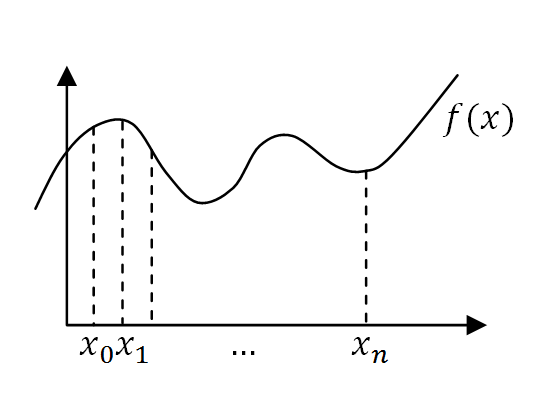
\includegraphics[scale=0.6]{l3_3.png}\\
    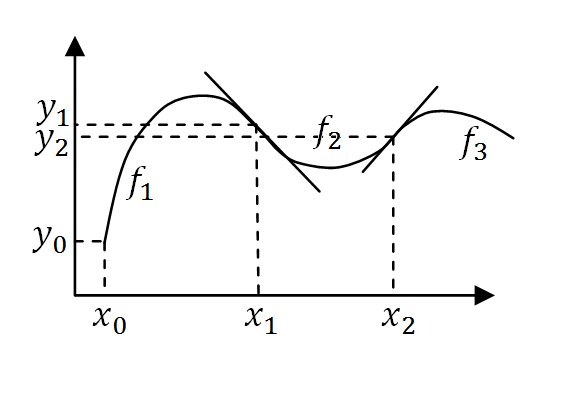
\includegraphics[scale=0.6]{l3_4.png}\end{center}
$  
\left\{  
\begin{array}{lcl}  
f_1'(x_0) = d_0 \\  
f_1(x_0) = y_0\\
f_1(x_1) = y_1\\
\end{array}   
\right.  
$
\\ \\
$  
\left\{  
\begin{array}{lcl}  
f_1'(x_1) = f_2'(x_1) \\  
f_2(x_1) = y_1\\
f_2(x_2) = y_2\\
\end{array}   
\right.  
$\\ \\
........... и т.д.\\
\\
\noindent \textbf{2. Кубический.}\\
$f_i(x)$ - кубическая парабола.\begin{center}
    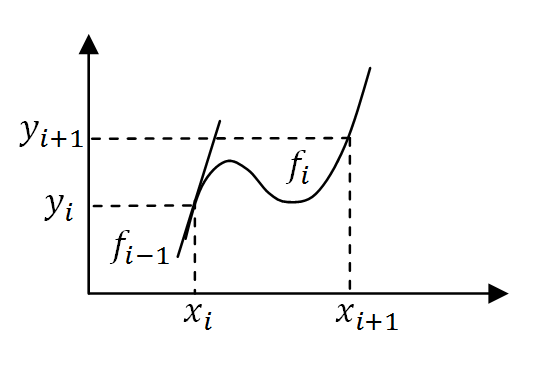
\includegraphics[scale=0.6]{l3_5.png}\end{center}
$  
\left\{  
\begin{array}{lcl}  
f_i(x_i) = y_i \\  
f_i(x_{i+1}) = y_{i+1}\\
f_i'(x_i) = f_{i-1}'(x_i)\\
f_i''(x_i) = f_{i-1}''(x_i)\\
\end{array}   
\right.  
$
\begin{center}
    $f_i(x) = a_0^i+a_1^ix+a_2^ix^2+a_3^ix^3 = a_i+b_i(x-x_i)+ \cfrac{c_i}{2}(x-x_i)^2+ \cfrac{d_i}{6}(x-x_i)^3$
\end{center}
\noindent \textbf{Пример 2.}
\begin{center}$f(x) = (x-1)(x-2)(x-3) = x^3-6x^2+11x-6$\end{center}
Аппроксимировать квадратичным сплайном с узлами $x_0=0, x_1=2, x_2=4$.\\ \\
$  
\left\{  
\begin{array}{lcl}
f(0)=(-1)\cdot (-2)\cdot (-3)=-6\\
f(2)=0\\
f(4)=6\\
\end{array}   
\right.  
$
\\ \\
$  
\left\{  
\begin{array}{lcl}
f_1 = a_0+a_1x+a_2x^2\\
f_1'(0) = a_1 = 11\\
f_1(0) = a_0 = -6\\
f_1(2) = -6+11\cdot 2+a_2\cdot 4 = 0 \Rightarrow a_2 = -4\\
\end{array}   
\right.  
$
\\ \\
Получим $f_1 = -6+11x-4x^2$. \\ \\
$  
\left\{  
\begin{array}{lcl}
f_1 = -6+11x-4x^2\\
f_2'(2) = f_1'(2) = -5\\
f_2(2) = 0\\
f_2(4) = 6\\
\end{array}   
\right.  
$
\\ ~\\
Подставим значения из предыдущих выражений.\\ \\
$
\left\{  
\begin{array}{lcl}
f_2 = b_0+b_1x+b_2x^2\\
b_0+2b_1+4b_2 = 0\\
b_1+4b_2 = -5\\
b_0+4b_1+16b_2 = 6\\
\end{array}   
\right.  
$
\\ \\
Получим $f_2 = 4x^2-21x+26$.\begin{center}
    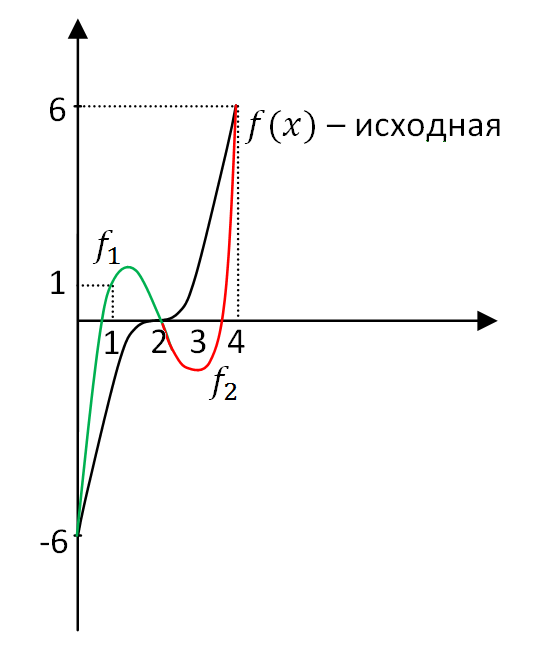
\includegraphics[scale=0.7]{l3_6.png}\end{center}

\subsection{Кривая Безье}
Есть набор из $n$ точек, хотим построить прямую, хорошо вписываемую в оболочку.\\
Параметризация отрезка для 2 точек, степень полинома $n = 1$:
\begin{center}
    $B(t) = (1-t)P_0+tP_1$\\
    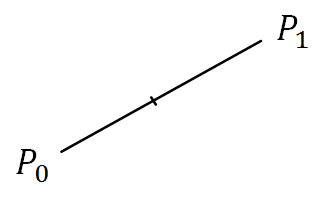
\includegraphics[scale=0.5]{l3_7.png}\end{center}
Параметризация отрезка для 3 точек, степень полинома $n = 2$.\\
Введем вспомогательные точки $M_1, M_2$ такие, что \begin{center}$M_1 = (1-t)P_0+tP_1$, $M_2 = (1-t)P_1+tP_2$\\
    $B(t) = (1-t)M_1+tM_2 = (1-t)^2P_0+2t(1-t)P_1+t^2P_2$\\
    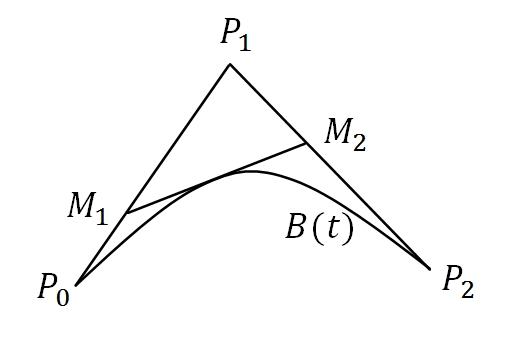
\includegraphics[scale=0.5]{l3_8.png}\end{center}
Параметризация отрезка для $n+1$ точек, степень полинома $n$.
\begin{center}$B(t) = \sum\limits_{k=0}^n C_n^k (1-t)^{n-k}t^kP_k$\end{center}
\noindent \textbf{Пример 3.}\\
Построить кубическую кривую Безье $B_3(t)$ для 4 точек, $t\in [0, 1]$.\begin{center}
    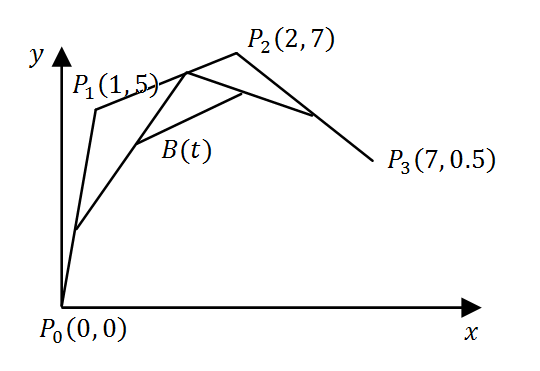
\includegraphics[scale=0.7]{l3_9.png}\end{center}
$x(t) = 1\cdot (1-t)^3\cdot t^0\cdot 0+3\cdot (1-t)^2\cdot t^1\cdot 1+3\cdot (1-t)^1\cdot t^2\cdot 2+(1-t)^0\cdot t^3\cdot 7 = 4t^3+3t$\\
$y(t) = 1\cdot (1-t)^3\cdot t\cdot 0+3\cdot (1-t)^2\cdot t\cdot 5+3\cdot (1-t)^1\cdot t^2\cdot 7+1\cdot (1-t)^0\cdot t^3\cdot \frac{1}{2} = - \frac{11}{2}t^3-9t^2+15t$\\ \\
\subsection{Домашнее задание 3}
\begin{enumerate}
    \item Приблизить следующую функцию $y(x)$ многочленом второй степени по методу наименьших квадратов:\\
    \begin{tabular}{|l|c|c|c|c|c|}
        \hline
        $x$ & -3 & -1 & 0 & 1 & 3 \\ \hline
        $y$ & -4 & -0.8 & 1.6 & 2.3 & 1.5\\ \hline
    \end{tabular}
    \item
    Доказать, что кривая Безье касается первого и последнего отрезка ломаной.
    \item
    Известно, что $f(x)$ --- многочлен третьей степени такой, что:\\ \\
    $
    \left\{
    \begin{array}{lcl}
    f(1) = 2 \\
    f(-1) = -3 \\
    f(2) = 17\\
    f(-2) = -19\\
    \end{array}
    \right.
    $\\
    \\Найти $f(x)$.
    \item
    Найти $f(x)$ многочлен наименьшей степени, удовлетворяющий условиям:\\ \\
    $
    \left\{
    \begin{array}{lcl}
    f(1) = -1 \\
    f'(1) = 5 \\
    f(0) = 0\\
    f'(0) = -1\\
    \end{array}
    \right.
    $
    \item
    Приблизить $sin~x$ сплайном $S(x)$ степени два с узлами $\pi k$, $\pi k + \cfrac{\pi}{2}$, $k\in \mathbb{Z}$. Найти $S \Big(\cfrac{\pi}{4} \Big)$, $S \Big(\cfrac{\pi}{3} \Big)$.
    \item На плоскости 100 точек, любые 4 из них лежат на параболе вида $y=ax^2+bx+c$. Доказать, что тогда все 100 точек будут лежать на одной и той же параболе.
\end{enumerate}
